% !TeX spellcheck = it_IT

\section{Algoritmi Distribuiti}

In un ambiente di calcolo distribuito, possiamo pensare alle entità di calcolo come nodi all'interno di un \textbf{grafo direzionato} $\vec G$, dove ogni arco indica un collegamento.\\

Ogni \textbf{entità possiede}:
\begin{itemize}
	\item Memoria locale
	\item Capacità di calcolo 
	\item Capacità di comunicazione
	\item \textbf{Clock locale}
\end{itemize} 

La differenza dal capitolo precedente è che i \textbf{processori sono asincroni}.\\

Nella memoria locale abbiamo: 
\begin{itemize}
	\item Registro di \textbf{input}: \texttt{valore($x$)}, input dell'entità $x$
	\item Registro di \textbf{stato} $=$ \texttt{stato($x$)}, stato dell'entità $x$; questo valore può essere cambiato localmente dalla stessa $x$
\end{itemize}

Per il \textbf{clock locale} è possibile settare o resettare una \textbf{sveglia}.\\
 \newpage

\paragraph{Proprietà delle entità:}
\begin{enumerate}
	\item \textbf{Reattive:} all'accadere di un "evento" compiono un'azione. Gli eventi possono essere:
	\begin{itemize}
		\item \textbf{Interni} al sistema: ricezione di messaggi, sveglia
		\item \textbf{Esterni} al sistema: impulso spontaneo (impulso di start)
	\end{itemize}
	L'entità sollecitata dall'evento risponde con un'azione: una \textbf{sequenza finita di operazioni indivisibili} (deve arrivare al termine).\\
	
	\item \textbf{Le entità seguono delle regole:} una \textbf{regola} è un oggetto della \textbf{forma} \texttt{stato $\times$ evento $\rightarrow$ azione}.\\
	Sia $x$ un'entità, allora $B(x)$ è l'\textbf{insieme delle regole a cui è soggetta} $x$. $B(x)$ deve essere \textbf{completo} (ogni coppia stato-evento deve avere un'azione specificata) e \textbf{non ambiguo} (con una singola interpretazione possibile).\\
	
	Se $E$ è un'\textbf{insieme di entità} che collaborano tra loro allora $B(E)$ è il \textbf{comportamento del sistema}
	$$ B(E) = \bigcup_{x \in E} B(x) $$
	è importante che $E$ sia \textbf{omogeneo}:
	$$ \forall x,y \in E, \;\;\;\;\; B(x) = B(y)$$
	Quando $B(E)$ è omogeneo viene chiamato \textbf{protocollo} per $E$ o \textbf{algoritmo distribuito} per E.\\
\end{enumerate}

\paragraph{Fact:} Sempre possibile ottenere $B(E)$ omogeneo.\\

\begin{proof}
	L'idea è di utilizzare un registro locale aggiuntivo che \textbf{differenzia} quelle \textbf{entità} che alla \textbf{stessa coppia stato-evento hanno azioni diverse}. Si usa
	\begin{itemize}
		\item \texttt{ruolo($x$)}: registro locale di $x$ che contiene il ruolo per $x$
	\end{itemize}
	
	La regola diventa:  \\
	\begin{tabular}{c c}
			\texttt{stato} $\times$ \texttt{evento} $\rightarrow$ \texttt{If ruolo(x)} & \texttt{then} $A_a$ \\ 
			& \texttt{else} $A_b$
	\end{tabular}
	\nn
\end{proof}

\newpage

\paragraph{Proprietà della rete: }
\begin{enumerate}
	\item La \textbf{comunicazione} tra entità \textbf{avviene usando link}, ed è importante che ogni entità conosca i propri collegamenti. Per ogni entità $x$, si ha un \textbf{etichettatura} denotata con $\lambda_x$ e dato che si trova in $\vec G$, si indicano con: 
	\begin{itemize}
		\item $N_{in} (x) =$ vicini in \textbf{ingresso} ad $x$
		\item $N_{out} (x) =$ vicini in \textbf{uscita} da $x$
	\end{itemize}
	
	\begin{center}
		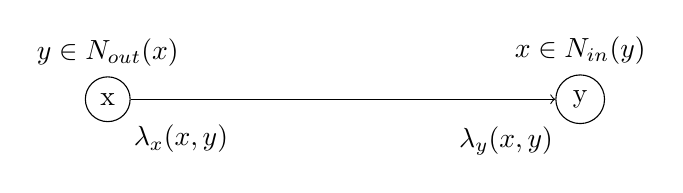
\begin{tikzpicture}
					\node[circle, draw, label=90:{$y \in N_{out} (x)$}, label=315:{$\lambda_x (x,y)$}] (x) at (0,0) {x}; 
					\node[circle, draw, label=90:{$x \in N_{in} (y)$}, label=225:{$\lambda_y (x,y)$}] (y) at (6,0) {y}; 
					\draw[->] (x) -- (y);
		\end{tikzpicture}
	\end{center}
	
	Per $x$ la funzione sarà $\lambda_x (x,y)$, mentre per $y$ l'etichettatura sarà $\lambda_y (x,y)$.\\
	
	\item \textbf{Assiomi di rete: }
	\begin{itemize}
		\item \textbf{Ritardo finito di comunicazione:} in assenza di errori, un messaggio spedito prima o poi arriverà
		\item \textbf{Orientamento locale:} ogni entità riesce a distinguere tra i suoi vicini $N_{in} (x)$ e $N_{out} (x)$ grazie alla conoscenza della funzione $\lambda_x$
	\end{itemize}
	\nn
\end{enumerate}

\paragraph{Parametri di rete: }
\begin{itemize}
	\item \textbf{Numero} di \textbf{entità} $n$ (nodi).\\
	
	\item \textbf{Numero} di \textbf{link} $m$ (archi).\\
	
	\item \textbf{Diametro} della rete $d$ (massima distanza tra due nodi).\\
\end{itemize}

\newpage

Oltre agli assiomi possiamo avere delle \textbf{restrizioni sulla rete}, da dichiarare al momento della scrittura del codice. Generalmente sono proprietà positive della rete, su cui fare affidamento.\\

\paragraph{Restrizioni sulla comunicazione:} 
\begin{itemize}
	\item \textbf{Link bidirezionali:} le connessioni tra le entità sono full duplex, si passa da un grafo diretto ad uno non diretto..\\
	$\forall x$, $N_{in} (x) = N_{out} (x) = N(x)$, quindi anche $\lambda_x (x, y) = \lambda_x (y, x)$.\\
	
	\item \textbf{Ordinamento dei messaggi:} i messaggi sullo stesso link vengono prelevati con politica FIFO (il primo inviato è il primo ad arrivare)
\end{itemize}

\paragraph{Restrizioni sull'affidabilità: }
\begin{itemize}
	\item \textbf{Rilevazione di errori:} ad esempio, quando cade un'entità o si guasta un canale di comunicazione.\\
	
	\item \textbf{Affidabilità parziale:} non ci saranno errori in futuro.\\
	
	\item \textbf{Affidabilità totale:} non ci sono stati errori e non ce ne saranno in futuro.\\
\end{itemize}

\paragraph{Restrizioni sulla topologia di rete: }
\begin{itemize}
	\item \textbf{Connettività del grafo:} $\vec G$ è fortemente connesso, $G$ è connesso.\\
\end{itemize}

\paragraph{Restrizioni sul tempo: }
\begin{itemize}
	\item \textbf{Tempi di comunicazione unitari:} la comunicazione impiega sempre un singolo ciclo di clock.\\
	
	\item \textbf{Clock sincronizzati:} come fosse un'architettura parallela a memoria distribuita.\\
\end{itemize}

\textbf{Nota:} tali restrizioni a volte vengono considerate per il calcolo delle prestazioni \textbf{ideali} del codice distribuito.\\

\newpage

%Slide 11
%End L19

\subsection{Misure di Complessità}

\paragraph{Tempo:} Viene considerato l'\textbf{intervallo} tra la \textbf{prima entità che si attiva} e l'\textbf{ultima che termina}. Esecuzioni diverse dello stesso codice può portare a tempi diversi in base alla congestione della rete.\\

Questo problema si risolve considerando il \textbf{tempo ideale}, si misura il tempo supponendo comunicazioni unitarie e clock sincroni.\\

Il tempo ideale si contrappone al \textbf{tempo causale} (caso peggiore), ovvero il tempo misurato considerando la catena più lunga di comunicazione richiesta dal codice; il peggiore di tutte le situazione che possono accadere.\\

\paragraph{Quantità di Comunicazione:} Si misura in termini di \textbf{numero di messaggi spediti}, se i messaggi sono omogenei/della stessa dimensione, altrimenti si valuta il \textbf{numero di bit spediti}.\\

\newpage

\subsection{Definizione di un Problema}

In genere un \textbf{problema} viene definito da una \textbf{tripla}: 
$$ P = <P_{init}, P_{final}, R> $$
Dove: 
\begin{itemize}
	\item $P_{init}$ e $P_{final}$ sono dei \textbf{predicati logici} che descrivono le \textbf{configurazioni del sistema all'inizio} (come sono inizializzati i registri all'interno delle entità all'inizio del protocollo) \textbf{e alla fine} (come devono essere i registri al termine).\\
	
	\item $R$ rappresenta le restrizioni del sistema, ad esempio full-duplex, no-errori, \dots\\
\end{itemize}

\textbf{Esempio di definizione} $P$ per \texttt{Broadcast}:
\begin{itemize}
	\item $P_{init}$: una sola entità detiene l'informazione $I$ e le altre identità non la hanno, i.e., 
	$$ \exists x \in E \; \text{ t.c. }\; valore(x) = I \; \wedge \; \forall y \neq x \;\; valore (y) = \emptyset $$
	
	\item $P_{final}$: tutte le entità posseggono $I$
	$$ \forall x \in E \;\;\; valore(x) = I $$
	
	\item $R$: link bidirezionali BL, totale affidabilità TR, connettività CN; queste 3 restrizioni si indicano con la sigla R; l'ultima restrizione è unico iniziatore UI; queste 4 restrizioni assieme si indicano con RI
\end{itemize}

\newpage

\subsection{Protocollo}

Un algoritmo distribuito, o \textbf{protocollo}, è un \textbf{insieme di regole della forma}: 
\begin{center}
	\texttt{stato $\times$ evento $\rightarrow$ azione}
\end{center}
Lo stato$_t (x)$ è lo stato dell'entità $x$ al tempo $t$. \\
L'evento può essere l'impulso spontaneo, la sveglia o la ricezione di un messaggio. \\
L'azione è un mini programma indivisibile che l'entità deve eseguire alla ricezione di un evento.\\

L'\textbf{esecuzione di un protocollo} è una \textbf{sequenza di configurazioni successive del sistema} (l'esecuzione porta a cambiamenti).\\

\paragraph{Definizione di configurazione:} Gli elementi che definiscono una configurazione sono:
\begin{itemize}
	\item $\Sigma (t)$: il \textbf{contenuto dei registri} delle entità al tempo $t$
	\item $Futuro(t)$: \textbf{eventi} già \textbf{generati} al tempo $t$ ma \textbf{non ancora processati} (messaggi inviati non arrivati, sveglie non ancora suonate, \dots)
\end{itemize}

Indichiamo la \textbf{configurazione del sistema} al tempo $t$ con $C(t)$
$$ C(t) = (\Sigma(t), Futuro(t))$$

Per esempio, la configurazione iniziale $C(0)$ è data dai registri inizializzati ($\Sigma(0)$) e dall'impulso spontaneo, presente ma non ancora processato ($Futuro(0)$).\\

L'\textbf{esecuzione del protocollo} distribuito viene descritta da una \textbf{sequenza di configurazioni successive}, tale che
$$ C(0) \xrightarrow{\text{ protocollo }} C(f)$$
Va dallo stato iniziale $C(0)$ allo stato finale $C(f)$.\\

\newpage

\paragraph{Notazione:} Quando una \textbf{configurazione} $C$ \textbf{soddisfa un predicato} $P$ scriveremo $C \in P$.\\

Bisogna \textbf{definire} come un protocollo distribuito \textbf{risolva un problema}.\\

\subsubsection{\texttt{Broadcast}}

\paragraph{Prima versione:} Riprendendo l'\textbf{esempio} del \texttt{Broadcast}: 
\begin{itemize}
	\item $P_{init}$: $\exists x \in E$ t.c. $valore (x) = I$ $\wedge$ $\forall y \neq x$ $valore (y) = \emptyset$
	\item $P_{final}$: $\forall x \in E$ $valore (x) = I$
	\item $R = $ RI $=$ (BL, TR, CN, UI)
\end{itemize}
Definendo due stati: 
$$ S = \{iniziatore, inattivo\} $$
E indichiamo con:
\begin{itemize}
	\item $S_{init}$ gli stati delle entità nella configurazione iniziale $C(0)$
	\item $S_{term}$ gli stati delle entità nella configurazione finale $C(f)$
\end{itemize}
Quindi, al termine vogliamo che tutte le entità siano sullo stato $inattivo$.\\

Le regole vengono specificate con stato, evento e azione, in quest'ordine, quindi: 
\begin{lstlisting}[escapeinside={(*}{*)}]
Iniziatore: 
	impulso spontaneo
	{	
		send(M) to N((*$x$*))
		become inattivo
	}
	
Inattivo: 
	ricezione(M)
	{	
		processa(M)
		send(M) to N((*$x$*))
	}
\end{lstlisting}

L'iniziatore manda a tutti i suoi vicini il dato, per poi diventare inattivo, mentre tutte le altre entità, alla ricezione del dato, lo inoltrano ai vicini.\\

Quindi possiamo ipotizzare che il messaggio $M$ sia una quadrupla: 
$$ M = (t, o, d, I)$$
Con: 
\begin{itemize}
	\item $t$: tipologia del messaggio
	\item $o$ e $d$: origine e destinazione
	\item $I$: informazione
\end{itemize}

%End VL 19

Ma c'è un problema: il protocollo è \textbf{corretto} (diffonde l'informazione tra tutte le entità) ma \textbf{non termina}. \\

Bisogna evitare di inviare il messaggio anche all'entità dalla quale è stato ricevuto. Inoltre, un'entità viene attivata anche se è già stata attivata in precedenza, formando cicli.\\

$Futuro(t) \neq \emptyset$, non c'è un momento senza messaggi in transito, quindi la comunicazione non termina.\\

La soluzione al problema è stabilire più stati, \textbf{raffinando gli stati}:
\begin{itemize}
	\item $S_{start} \subseteq S_{init}$: stati che fanno iniziare il protocollo
	\item $S_{final} \subseteq S_{term}$: stati per cui la \textbf{sola azione è quella nulla} 
\end{itemize}
Per \texttt{Broadcast}, $S_{start} = \{iniziatore\}$ mentre $S_{init} = \{iniziatore, inattivo\}$, per gli stati finali ne introduciamo uno nuovo: $S_{term} = S_{final} = \{finito\}$. 3 stati totali.\\

Grazie all'uso dello stato "$finito$" il protocollo riesce a terminare. Dopo essere $inattivo$ un'entità entra nello stato $finito$, non rimane più nello stesso stato.\\

\newpage

\textbf{Formalmente}, possiamo dire che la soluzione per $P$: 
\begin{itemize}
	\item è \textbf{corretta} se
	$$ \forall C(0) \in P_{init} \;\;\; \exists t'  \; \text{ t.c. } \; \forall t > t' \;\; C(t) \in P_{final} $$
	per ogni condizione iniziale, a un certo punto si arriva a una delle configurazioni finali.\\
	
	\item \textbf{Termina} se
	$$ \forall x \in E \;\;\; stato_t (x) \in S_{final} $$
	ogni entità presente è in uno stato finale.\\
\end{itemize}

Devono valere entrambe.

\paragraph{Seconda versione (Flooding):} Gli stati sono
$$ S = \{iniziatore, inattivo, finito\} $$
$$ S_{start} = \{iniziatore\} $$
$$ S_{final} = \{finito\}$$
L'iniziatore fa partire il protocollo, le entità nello stato finito non eseguono più operazioni.\\
Codice:
\begin{lstlisting}[escapeinside={(*}{*)}]
	Iniziatore: 
	impulso spontaneo
	{	
		send(M) to N((*$x$*))
		become finito
	}
	
	Inattivo: 
	ricezione(M)
	{	
		processa(M)
		send(M) to N((*$x$*)) - sender
		become finito
	}
\end{lstlisting}
Le coppie stato-evento non indicate eseguono azione nulla.\\

\newpage

\paragraph{Complessità:}
\begin{itemize}
	\item \textbf{Numero di messaggi} $M$:
	$$ M[Flooding] = \sum_{x \in E} (N(x) - 1) + 1 = 2m - n + 1$$
	Dove $m$ è il numero di archi e $n$ il numero di nodi. Fa mandare il messaggio a tutti i vicini, eccetto il sender.\\
	
	\item \textbf{Tempo} $T$: 
	$$ T[Flooding] \leq d $$
	Dove $d$ è il diametro della rete. Per questo calcolo si suppone clock sincroni e ritardo unitario per la consegna dei messaggi. Il tempo è pari al diametro nel caso peggiore, può essere meno.\\
\end{itemize}

\textbf{Lower bound} del problema: 
\begin{itemize}
	\item \textbf{Tempo causale} (caso peggiore) per il problema
	$$ T[BCast/RI] \geq d$$
	Non si possono impiegare meno di $d$ passi.\\
	
	\item \textbf{Numero di messaggi}, c'è un teorema che dice
	$$ M[BCast/RI] \geq m$$
	Non si può scendere sotto $m$.\\
\end{itemize}

Flooding è quindi ottimale ($2m$ messaggi, lineare) per il problema di \texttt{Broadcast}.\\

\newpage

\paragraph{Teorema:} $M[BCast/RI] \geq m$.\\

\begin{proof}
	Per assurdo, risolvo il problema con meno di $m$ messaggi. Vuol dire che esiste un arco su cui non viaggiano messaggi. Sia $A$ il protocollo che non manda il messaggio sull'arco $(x,y)$. Se $A$ è corretto deve lavorare bene su ogni $G$.\\
	
	Creo il grafo $G'$ aggiungendo un nodo $z$ tra $x$ e $y$, rimuovendo l'arco $(x,y)$ e aggiungendo $(x,z)$ e $(z,y)$. Cambio le etichettature $\lambda_x (x,z) = \lambda_x (x,y)$ e $\lambda_y(y,z) = \lambda_y (y,z)$.\\
	
	\begin{center}
		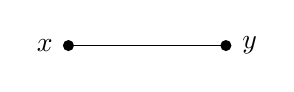
\begin{tikzpicture}
			\node (1) at (-0.3,0) {$x$};
			\node (2) at (2.3,0) {$y$};
			
			\draw[-] (0,0) -- (2,0);
			\fill (0,0) circle (2pt);
			\fill (2,0) circle (2pt);
		\end{tikzpicture}
		\nn \nn
		$\Downarrow$
		\nn \nn
		\begin{tikzpicture}
			\node (1) at (-0.3,0) {$x$};
			\node (2) at (2.3,0) {$y$};
			\node (2) at (1,-2.3) {$y$};
			
			
			\draw[dashed] (0,0) -- (2,0);
			\draw[-] (0,0) -- (1,-2);
			\draw[-] (2,0) -- (1,-2);
			\fill (0,0) circle (2pt);
			\fill (2,0) circle (2pt);
			\fill (1,-2) circle (2pt);
		\end{tikzpicture}
	\end{center}
	
	Se eseguo il protocollo $A$ su $G'$ il nodo $z$ non riceve $I$, dato che sull'arco $(x,y)$ non viaggiava nessun messaggio questo accade anche su $(x,z)$, quindi $A$ non è corretto.\\
\end{proof}

\newpage

\subsection{Problema \texttt{Wake-Up}}

Nel problema \texttt{Broadcast}, c'era una singola entità che doveva raggiungere tutte le altre, mentre per \texttt{Wake-up} possono esserci più entità che iniziano il protocollo. Si rilassa il vincolo di unico iniziatore UI. Ci sono entità "dormienti" e altre che sono "sveglie", bisogna svegliarle tutte.\\

\subsubsection{Protocollo WFlood}
Stati
$$ S = \{dormiente, attivo\} $$
$$ S_{init} = \{dormiente\} = S_{start} $$
$$ S_{term} = \{attivo\} = S_{final} $$

Ora però l'impulso spontaneo può arrivare a un certo numero di entità.\\

\begin{lstlisting}[escapeinside={(*}{*)}]
Dormiente:
	impulso spontaneo
	{
		send(W) to N(x)
		become attivo
	}
	ricezione(W)
	{
		send(w) to N(x) - sender
		become attivo
	}
\end{lstlisting}

Ci può essere l'impulso spontaneo oppure la ricezione di un messaggio per passare allo stato attivo.\\

\newpage

\paragraph{Costo:}
\begin{itemize}
	\item \textbf{Tempo}: 
	$$ T[WFlood] \leq d $$
	Dove $d$ è il diametro.\\
	
	\item \textbf{Numero di messaggi}:
	$$ 2m - n + 1 \leq M[WFlood] \leq 2m $$
	Il bound inferiore è se una sola entità si attiva, mentre il $2m$ è il caso in cui si attivano tutte.\\
\end{itemize}

%End VL 20, End slide 20

\newpage

\subsection{Problema \texttt{Traversal}}

Ogni entità della rete deve essere visitata, ma \textbf{sequenzialmente}, ovvero una dopo l'altra.\\
Risulta utile in ambito di gestione condivisa delle risorse.\\

La configurazione iniziale è che tutti i nodi sono $unvisited$, tranne uno.\\

\subsubsection{\texttt{Depth-First Traversal}}

Il protocollo da definire sarà \texttt{Depth-First Traversal}, equivalente alla visita in profondità di un grafo; si scende sempre verso il vicino non ancora visitato.\\

Idea: viene usato un messaggio particolare \textbf{Token} $T$. Quando un nodo riceve il token $T$ diventa $visited$, ma ad ogni istante di tempo viaggia \textbf{al più un solo} $T$.\\

\textbf{Passaggi} principali dell'algoritmo: 
\begin{enumerate}
	\item Un nodo che \textbf{riceve} $T$ per la \textbf{prima volta} deve: 
	\begin{itemize}
		\item ricordarsi il sender (non dovrà rinviargli il token)
		\item fare una \textbf{lista dei vicini non visitati} (ma non lo sa, per ora tutti eccetto il sender)
		\item invia $T$ ad uno di essi
		\item aspetta un messaggio da quest'entità, che può essere \texttt{return} o \texttt{back-edge}
	\end{itemize}
	\nn
	
	\item Il \textbf{vicino che riceve} $T$:
	\begin{itemize}
		\item se è il \textbf{primo} $T$ che riceve, va al \textbf{passaggio 1}
		\item altrimenti, se è \textbf{già stato visitato}, spedisce un \texttt{back-edge}
	\end{itemize}
	\nn
	
	\item Solo dopo aver \textbf{finito la lista dei vicini non visitati} deve inviare un \texttt{return} al sender.\\
\end{enumerate}

\newpage

Quindi sono presenti \textbf{3 tipi di messaggi}:
\begin{itemize}
	\item \texttt{Token} $T$
	\item \texttt{Back-edge} $B$
	\item \texttt{Return} $R$
\end{itemize} 

\paragraph{Protocollo:} Stati:
$$ S = \{initiator, idle, visited, done\}$$
$$ S_{init} = \{initiator, idle\} $$
$$ S_{term} = \{done\}$$

Codice: 
\begin{lstlisting}[escapeinside={(*}{*)}]
Initiator
	Spontaneously
	{
		initiator = true
		unvisited = N((*$x$*))
		visit
	}
	
Idle
	Receive (T)
	{
		entry = sender
		unvisited = N(x) - sender
		initiator = false
		visit
	}
\end{lstlisting}
	
\newpage
	
\begin{lstlisting}[escapeinside={(*}{*)}]
Procedure visit
{
	if unvisited (*$\neq \emptyset$*) then 
		next (*$\leftarrow$*) unvisited
		send(T) to next
		become visited
	else 
		if initiator = false then 
			send(return) to entry
		become done
}

Visited
	Receiving(return)
	{
		visit
	}
	Receiving(back-edge)
	{
		visit
	}
	Receiving(T)
	{
		unvisited = unvisited - sender
		send(back-edge) to sender
	}
\end{lstlisting}

\paragraph{Complessità:} Osservazione: su ogni link deve viaggiare il \texttt{token} ed in risposta ci sarà un \texttt{return} o \texttt{back-edge}. Il tutto avviene praticamente in maniera \textbf{sequenziale}.\\

Quindi il \textbf{tempo coincide con i messaggi}
$$ T[DF-Traversal] = M[DF-Traversal] = 2m $$

\newpage

\paragraph{Lower bound al problema \texttt{Traversal}:}
\begin{itemize}
	\item $M[Traversal] \geq m$, vale lo stesso teorema visto per il Broadcast
	\item $T[Traversal] \geq n-1$, dato che ogni nodo deve essere visitato in sequenza
\end{itemize}


Nel caso di un grafo connesso, il \textbf{numero di archi} $m$ è
$$ n-1 \leq m \leq \frac{n(n-1)}{2} = O(n^2)$$

Di conseguenza DF-Traversal:
\begin{itemize}
	\item è \textbf{ottimo} per il \textbf{numero di messaggi}
	\item ma nel caso peggiore \textbf{NON per il tempo} ($n$)
\end{itemize}

\paragraph{Osservazione:} Il problema per il costo del tempo è che ad ogni istante di tempo \textbf{viaggia un messaggio $T$ solo}.\\

La soluzione è introdurre concorrenza, aggiungendo messaggi in quantità opportuna ($O(m)$).\\

Possiamo evitare di inviare $T$ su un link \texttt{back-edge}? \\
Idea: un nodo \textbf{non visitato} che \textbf{riceve} $T$ \textbf{comunica} l'evento ai \textbf{vicini} mandando un \textbf{messaggio} \texttt{visited} (in contemporanea con $T$), i vicini che ricevono \texttt{visited} aggiornano la propria lista unvisited.\\

Ma questo risolve il problema di inviare $T$ su \texttt{back-edge}? Non completamente, si può vedere in casi di ritardo della comunicazione, in cui il \texttt{visited} impiega tempo ad arrivare.\\

Ma quando un entità "capisce l'errore" e riceve un \texttt{visited}, spedisce $T$ ad un'altra entità, oppure invia un \texttt{return} e sarà l'entità che lo riceve a spedire un altro $T$.\\

Inoltre, se un nodo riceve $T$: lo interpreta come fosse un \texttt{back-edge} ed elimina il nodo dalla lista di unvisited, in quanto sicuramente è già stato visitato.

\newpage

\paragraph{Nuova complessità:}
\begin{itemize}
	\item \textbf{Messaggi}:
	$$ 
	\begin{array}{c c}
		2n-2 & \leftarrow T + R \\
		2m - (n-1) & \leftarrow visited \\
		2(m-(n-1)) & \leftarrow \text{errori di invio di } T \\
		\implies O(m) & \text{totale}
	\end{array}
	$$
	
	\item \textbf{Tempo}: considerando tempo ideale senza ritardi nè errori. Inoltre i \texttt{visited} son in sovrapposizione con $T$. Totale:
	$$ 2(n-1) = O(n) $$
\end{itemize}

Chiamando il protocollo modificato $DF^\ast$, questo è \textbf{ottimo} per
\begin{itemize}
	\item Quantità di \textbf{messaggi} $M[DF^\ast] = O(n)$
	\item \textbf{Tempo} ideale $T[DF^\ast] = O(n)$
\end{itemize}

In quanto rispetta i lower bound.\\

\vfill

Codice non richiesto all'esame, non lo riporterò, definisce il protocollo $DF^\ast$.\\

% End L21

\newpage

\subsection{Problema \texttt{Spanning Tree}}

I problemi \texttt{Broadcast}, \texttt{Wake up} e \texttt{Traversal} hanno una \textbf{complessità di messaggi} che è $\Theta (m)$, dove $m$ è il numero di link e $n$ il numero di entità.\\

Quindi la \textbf{complessità varia} in base alla \textbf{topologia del grafo}
$$ n-1 \leq m \leq \frac{n(n-1)}{2} $$

$n-1$ è il minimo numero di link per collegare $n$ entità, come in un albero, mentre l'estremo opposto è un grafo completamente connesso.\\

\paragraph{Idea:} Quindi per \textbf{minimizzare} la \textbf{complessità di comunicazione} si potrebbe \textbf{utilizzare una sottorete} al posto dell'intero grafo $G$, e la sottorete minima è quella generata da uno \textbf{spanning tree}. Poi si possono risolvere gli altri problemi sullo spanning tree.\\

Il \textbf{costo} per risolvere i problemi diventa somma di: 
\begin{itemize}
	\item \textbf{costo} di \textbf{costruzione} dell'\textbf{albero} 
	\item \textbf{costo originale} del problema eseguito sull'albero
\end{itemize}

Ad esempio, il costo di \texttt{Broadcast} con algoritmo Flooding su uno spanning tree di $n$ entità è esattamente $n-1$ messaggi.\\

Problema dello \texttt{Spanning Tree}: vogliamo \textbf{costruire una sottorete} tale che: 
\begin{itemize}
	\item coinvolga \textbf{tutte le entità}
	\item le entità siano \textbf{connesse}
	\item \textbf{priva di cicli}
\end{itemize}

Risolvere un algoritmo distribuito sulla sottorete richiede di tenere conto del fatto che l'algoritmo deve essere a \textbf{conoscenza dell'albero su cui viene eseguito}. \textbf{Ogni entità} vedrà (tiene traccia di) una \textbf{piccola parte dell'albero}.\\

\newpage

\paragraph{Notazione:} 
\begin{itemize}
	\item $\forall x \in E$ definiamo 
	$$ Tree\_N(x) \subseteq N(x) $$
	sottoinsieme che contiene i \textbf{vicini} di $x$ \textbf{all'interno dell'albero}.\\
	
	\item L'insieme dei \textbf{lati} per l'albero:
	$$ (x,y) \in link(Tree\_N(x)) \Leftrightarrow y \in Tree\_N (x) $$
	quindi un lato $(x,y)$ è all'interno di $link(Tree\_N(x))$ solo se $y \in Tree\_N (x)$.\\
	
	\item L'\textbf{intero albero} è
	$$ Tree = \bigcup_{x \in E} link(Tree\_N(x)) $$
	ovvero, l'unione di tutti i collegamenti per ogni nodo.\\
\end{itemize}

Risolviamo il problema \texttt{Spanning Tree} con le \textbf{restrizioni RI} (Bidirectional Link, Total Reliability, Connectivity, Unique Initiator).\\

Il protocollo che risolve il problema dello \texttt{Spanning Tree} si chiama \texttt{Shout}:
\begin{itemize}
	\item ogni \textbf{entità vede} solo i suoi $Tree\_N(x)$
	\item e tiene traccia del \textbf{padre}
\end{itemize}

La \textbf{radice} dell'albero è data dall'\textbf{entità che inizia} il protocollo.\\

La strategia di \texttt{Shout} è chiedere ai vicini se questi vogliono diventare vicini anche nell'albero.\\

\newpage

\textbf{Schema}: 
\begin{itemize}
	\item L'iniziatore $s$ (root) \textbf{spedisce} la \textbf{domanda} $Q$ ai suoi \textbf{vicini} e attende le risposte (chiede se vogliono diventare figli).\\
	
	\item Ogni entità $x \neq s$ che \textbf{riceve} $Q$:
	\begin{itemize}
		\item la \textbf{prima volta} risponde "\textit{yes}" (viene connessa all'albero) e \textbf{invia} $Q$ ai suoi vicini e si mette in attesa
		\item le \textbf{volte successive} risponde "\textit{no}" (già connessa)
	\end{itemize}
	\nn
	
	\item Inoltre serve \textbf{memorizzare l'entità padre} e le \textbf{entità che rispondono} "\textit{yes}".\\
	
	\item L'entità \textbf{termina quando riceve tutte le risposte}.\\
\end{itemize}

\texttt{Shout} è sostanzialmente un Flooding $+$ Reply. Si diffonde un messaggio $Q$ a cui bisogna rispondere "\textit{yes}" o "\textit{no}".\\

\textbf{Linee guida} per definire il codice:
\begin{itemize}
	\item Tre \textbf{tipi di messaggi}: $Q$, $yes$, $no$.\\
	
	\item Ogni entità ha la \textbf{visibilità locale del proprio} albero, quindi bisogna \textbf{aggiornare le variabili locali}: $root$ (bool per indicare se è la radice), $parent$ (tiene traccia del padre, uno dei nodi all'interno della lista), $Tree\_N(x)$ (lista di vicini di albero), $counter$ (conta il numero di risposte ricevute a $Q$, permette di terminare correttamente).\\
	
	\item \textbf{Aggiornare lo stato}, vanno utilizzati in maniera corretta per raggiungere la terminazione.\\
\end{itemize}

\newpage

\subsubsection{Protocollo \texttt{Shout}}
Gli \textbf{stati} sono:
$$ S = \{iniziatore, inattivo, attivo, finito \} $$
$$ S_{init} = \{iniziatore, inattivo \} $$
$$ S_{final} = \{finito\} $$

Nella configurazione iniziale ci sarà un solo $iniziatore$ e tutte le altre entità $inattive$, che diventeranno $attive$ quando ricevono il primo $Q$, e ci rimarranno fino al momento in cui a loro volta non riceveranno tutte le risposte, diventando $finite$.\\

Bisogna definire le azioni per $iniziatore$, $inattivo$, $finito$.\\

Per quanto riguarda l'iniziatore:
\begin{lstlisting}[escapeinside={(*}{*)}]
Iniziatore
	Impulso spontaneo
	{
		root = true
		counter = 0 
		Tree_N((*$x$*)) = (*$\emptyset$*)
		send(Q) to N((*$x$*))
		become attiv
	}
\end{lstlisting}

\newpage

Ogni inattivo:
\begin{lstlisting}[escapeinside={(*}{*)}]
Inattivo 
	Ricezione(Q)
	{
		root = false
		parent = sender 
		counter = 1
		Tree_N((*$x$*)) = {sender}
		send("yes") to sender
		if counter = |N((*$x$*))| then 
			become finito
		else 
		{
			send(Q) to N(x)\sender
			become attivo
		}
	}
\end{lstlisting}

Ogni attivo:
\begin{lstlisting}[escapeinside={(*}{*)}]
Attivo
	Ricezione(Q)
	{ send("no") to sender }
	Ricezione("yes")
	{
		Tree_N((*$x$*)) = Tree_N((*$x$*)) (*$\cup$*) {sender}
		counter = counter + 1
		if counter = |N((*$x$*))| then 
			become finito
	}
	Ricezione("no")
	{
		counter = counter + 1
		if counter = |N((*$x$*))| then 
			become finito
	}
\end{lstlisting}

\newpage

\paragraph{Correttezza di \texttt{Shout}:}
\begin{itemize}
	\item \textbf{Terminazione:} in assenza di errori, viene sempre ricevuto un numero di risposte pari ai $Q$ inviati, diventando finito.\\
	
	\item \textbf{Tutte le entità presenti:} grazie al Flooding di $Q$.\\
	
	\item \textbf{Le entità sono connesse:} grazie al fatto che al primo $Q$ rispondo "$yes$".\\
	
	\item \textbf{Privo ci cicli:} ogni entità risponde solo una volta con "$yes$" (tranne la radice, che risponde sempre "$no$")
\end{itemize}

\paragraph{Costo:}
\begin{itemize}
	\item \textbf{Numero di messaggi}: 
	$$ M[Shout] = 2M[Flooding] = 2[2m - (n-1)] \sim 4m $$
	
	\item \textbf{Tempo:}
	$$ T[Shout] = T[Flooding] + 1 \leq d + 1 $$
\end{itemize}

I \textbf{lower bound} per questo problema SPT sono: 
$$ M[SPT/RI] \geq m $$
$$ T[SPT/RI] \geq d $$
Quindi abbiamo un protocollo \textbf{ottimale} $O(m)$ per i messaggi e $d+1$ per il tempo.\\

\newpage

\subsubsection{\texttt{Shout} migliorato: \texttt{Shout+}}

Per quanto riguarda il tempo non si può migliorare, ma posso \textbf{ridurre il numero di messaggi} (abbiamo un 4 come coefficiente)? I messaggi
\begin{itemize}
	\item di "$yes$" sono necessari
	\item di "$no$" possono essere eliminati
\end{itemize}

Se la risposta è un "$no$" è perché l'entità ha già ricevuto in precedenza un $Q$ a cui ha risposto "$yes$", inviando contestualmente altri $Q$.\\

Quindi una entità attiva che \textbf{riceve un} messaggio $Q$ può \textbf{interpretare} quest'ultimo \textbf{come un} "$no$".\\

Questo rimuove la necessità di rispondere "$no$", su ogni arco viaggerà una richiesta $Q$ e una risposta, la quale può essere "$yes$" oppure un altro $Q$.\\

\paragraph{Nuovo costo di comunicazione:}
$$ M[Shout+] = 2m $$ 

Su \textbf{ogni link} viaggiano: 
\begin{itemize}
	\item o un $Q$ seguito da $yes$
	\item o un $Q$ seguito da un $Q$
\end{itemize}

\vfill 

\paragraph{Altra soluzione per lo spanning tree:} Utilizzare il protocollo \texttt{Traversal}. Un arco fa parte dell'albero se su quel link passa un \texttt{return}, si costruisce l'albero in maniera sequenziale (tendenzialmente peggio di \texttt{Shout} che lo fa in parallelo).\\

% End L22

\newpage

\subsection{Problema \texttt{Election}}

"Rompere la simmetria", lo scopo è \textbf{individuare un'entità specifica} tra tante entità autonome e omogenee. Tale entità sarà chiamata \texttt{leader}, le altre \texttt{follower}. Bisogna fare una scelta.\\
Per certe applicazioni serve avere un'unità centrale che diventi coordinatrice per altre entità.\\

Se le entità sono \textbf{omogenee} la scelta del leader diventa \textbf{difficile}.\\

\paragraph{Fact:} Impossibile \textbf{individuare deterministicamente} un leader sotto le restrizioni R (ovvero entità omogenee e unico initiator).\\

Idea della dimostrazione: Siano $x,y \in E$ entità omogenee. Esse sono nello \textbf{stesso stato} e \textbf{inizializzate nello stesso modo}. Eseguono lo stesso algoritmo e di conseguenza lo stesso codice. Partono in simmetria, eseguono lo stesso codice e \textbf{rimarranno sempre simmetriche}.\\

Quindi sotto le restrizioni RI: la starting entity diventa immediatamente leader.\\
Ma questa è una soluzione che "viene dall'esterno", ma vogliamo che il leader sia scelto dalle entità stessse.\\

\subsubsection{Initial Distinct Values ID}

Introduciamo una \textbf{nuova restrizione}: \textbf{Initial Distinct Values (ID)}. Forniamo un \textbf{nome ad ogni entità}, $id(x) =$ nome di $x \in E$, o valore di $x$.\\

Notazione: $R \cup \{ID\} = IR$.\\

\newpage

\paragraph{Strategie di soluzione:}
\begin{enumerate}
	\item \textbf{Elect minimum} 
	\begin{itemize}
		\item si trova l'entità con $id(x)$ minimo che diventerà \texttt{leader}
		\item tutte le altre, $\forall y \neq x \in E$ , diventano \texttt{follower}
	\end{itemize}
	\nn
	
	\item \textbf{Elect minimum initiator}
	\begin{itemize}
		\item trova $id(x)$ minimo tra le sole entità \texttt{initiator} ed elegge a \texttt{leader}
		\item $\forall y \neq x \in E$, $y$ diventa \texttt{follower} (tutte le altre)
	\end{itemize}
\end{enumerate} 


\paragraph{Topologia di rete:} Risolviamo il problema in una topologia particolare: \textbf{Ring-Anello}.\\
Le entità sono disposte ad anello, nel caso $m=n$
$$ A = (x_0, x_1, \, \dots \, , x_{n-1}) $$
\begin{center}
	\begin{tikzpicture}[scale=0.8]
		\node[circle, draw, minimum width=1cm, minimum height=1cm, inner sep=0] (1) at (0,0) {$x_0$};
		\node[circle, draw, minimum width=1cm, minimum height=1cm, inner sep=0] (2) at (3,-2) {$x_1$};
		\node[circle, draw, minimum width=1cm, minimum height=1cm, inner sep=0] (3) at (-3,-2) {$x_{n-1}$};
		\node (4) at (-2.75, -3.5) {};
		\node (5) at (2.75, -3.5) {};
		
		% Draw bent arrows 
		\draw[-, bend left=30] (1) to (2);
		\draw[-, bend right=30] (1) to (3);
		
		\draw[dashed, bend right=10] (3) to (4);
		\draw[dashed, bend left=10] (2) to (5);
	\end{tikzpicture}
\end{center}

Ogni entità è \textbf{collegata} a quella \textbf{precedente} e quella \textbf{successiva}, dove $x_0$ è la successiva di $x_{n-1}$ e viceversa.\\

\paragraph{Restrizioni:} $IR \cup \{x \in A$ sa di essere in un anello$\}$.\\

\paragraph{Notazione:} $N(x) -$ \texttt{sender} è detto \texttt{other} (sono solo 2, se non è il \texttt{sender} è l'altro).\\

\newpage

\subsubsection{Protocollo \texttt{All The Way}}

I messaggi viaggiano intorno all'anello, inoltrati dalle entità sempre nella stessa direzione.\\

\textbf{Formato} dei messaggi: 
$$(Elect, id(x), \, \dots)$$

Supponendo di avere $x,y,z$ collegate in quest'ordine. Quando $x$ riceve il messaggio $M$:
\begin{itemize}
	\item inoltra $M$ 
	\item invia un messaggio $M' = (Elect, id(x), \, \dots)$ verso \texttt{other}, con il proprio id
\end{itemize}

In questo modo \textbf{ogni entità} $x \in E$ \textbf{vede gli id di tutte le altre entità}, $id(y)$, $\forall y \neq x \in E$, e può calcolare il minimo. Sull'anello viaggia ogni id.\\

\textbf{Quando far terminare una entità?} Una volta che $x$ \textbf{riceve} un \textbf{messaggio} contenente \textbf{il proprio id} il messaggio ha fatto il giro dell'anello, quindi non lo inoltra più.\\

Può $x$ terminare? 
\begin{itemize}
	\item \textbf{sì:} solo se si suppone la restrizione "Message ordering", ovvero che i messaggi vengono prelevati con politica FIFO, ma noi non abbiamo questa restrizione.\\
	
	\item \textbf{solo se ha già visto $n$ messaggi:} si suppone che le entità siano a conoscenza della dimensione dell'anello, altra restrizione che non abbiamo.\\
	
	\item \textbf{no:} bisogna completare l'ultimo campo del messaggio $M$ (quello con i puntini) per far terminare correttamente le entità.\\
\end{itemize}

\newpage

Aggiungiamo un \textbf{contatore}: 
$$ M = (Elect, id(x), counter) $$

Ma \textbf{come usarlo}? 
\begin{itemize}
	\item inizialmente l'entità $x$ pone \texttt{counter} $=1$
	\item ogni altra entità $y \neq x \in E$ somma 1 a \texttt{counter}
	\item quando $M$ torna ad $x$ \texttt{counter} deve essere pari a $n = |A|$, ovvero la \textbf{dimensione dell'anello}
\end{itemize}

Quindi se $x$ ha già \textbf{ricevuto} $n$ \textbf{diversi id può terminare}, altrimenti \textbf{aspetta di ricevere $n$ id diversi}.\\

Gli \textbf{stati} sono:
$$ S = \{asleep, awake, leader, follower\}$$
$$ S_{init} = \{asleep\} $$
$$ S_{final} = \{leader, follower\}$$

All'inizio ogni nodo è:
\begin{lstlisting}[escapeinside={(*}{*)}]
Asleep
	Spontaneously
	{
		Initialize 
		become awake
	}
	Receving(Elect, value, counter)
	{
		send(Elect, value, counter+1)
		min=Min(min, value)
		count=count+1
		become awake
	}
\end{lstlisting}

\newpage

Procedura \texttt{Initialize}
\begin{lstlisting}[escapeinside={(*}{*)}]
Procedure Initialize
	{
		count=0
		size=1
		know=false
		send(Elect, id((*$x$*)), size) to right
		min=id((*$x$*))
	}
	
Awake
	Receiving(Elect, value, counter)
	{
		if value!=id then
		{
			send(Elect, value, counter+1) to other
			min=Min(min, value)
			count=count+1
			if know=true then Check
		} else
		{
			size=counter
			know=true
			Check
		}
	}
	
Procedure Check
	{
		if count=size then
		{
			if min=id((*$x$*)) then 
				become leader
			else
				become follower
		}
	}
\end{lstlisting}

\newpage

\paragraph{Complessità: }
\begin{itemize}
	\item \textbf{Numero di messaggi:} 
	$$ M[AllTheWay/RI \cup Ring] = n^2$$
	ogni entità invia/inoltra $n$ messaggi.\\
\end{itemize}

Ma questo è \textbf{troppo costoso}, quindi passiamo alla strategia \textbf{Elect Minimum Initiator}: solo gli \texttt{initiator} \textbf{generano} $M$, tutti gli altri inoltrano e basta.\\

\textbf{Problema di terminazione}: per le \textbf{entità non} \texttt{initiator}, non vengono a conoscenza di $n$ non ricevendo il proprio messaggio. \\
Quando è terminato il calcolo del leader da parte degli \texttt{initiator}, il \textbf{\texttt{leader} deve mandare un messaggio di fine} agli altri: si aggiungono \textbf{$n$ messaggi di fine}.\\

\paragraph{Nuova Complessità:}
\begin{itemize}
	\item \textbf{Numero di messaggi:}
	$$ M[AllTheWay - MinInitiator] = n \cdot k + n $$
	dove $k$ è il numero degli \texttt{initiator}. Ogni messaggio fa il giro dell'anello, più i messaggi di fine.\\
	
	\item \textbf{Tempo:}
	$$ T[AllTheWay - MinInitiator] \leq 3n - 1 $$
	ed il bound è raggiungibile con $2$ \texttt{initiator} che si svegliano in momenti diversi. Ci sono $n$ messaggi ed $n$ passaggi per ognuno dei 2 \texttt{initiator}, poi $n-1$ messaggi di fine inviati dal \texttt{leader}.\\
\end{itemize}

%End L23

\newpage

\subsection{Problema \texttt{Routing}}
L'entità $x$ vuole mandare un messaggio all'entità $y$ e vuole sapere il percorso, ovvero \textbf{individuare un cammino} in $\vec{G}$ da $x$ a $y$.\\

Per risolverlo potrebbe essere sufficiente usare il \texttt{Broadcast}, da $x$ a tutte le altre entità. Ma questo è, ovviamente, molto inefficiente.\\

Allora \textbf{scegliamo un cammino tra i tanti possibili} tra $x$ e $y$, senza preoccuparci di che cammino sia, ma se è il migliore, meglio.\\

\subsection{Problema \texttt{Shortest Path}}
Determinare il \textbf{cammino di costo minimo} tra $x$ e $y$ in $\vec{G}$.\\
Ha molte applicazioni in ambito di comunicazione, cruciale in una computazione di un sistema distribuito.\\

Richiede di usare memoria e informazioni sui costi di $\vec{G}$ per ogni entità $x \in E$, al fine di \textbf{calcolare i cammini minimi verso ogni altra entità}.

\paragraph{Restrizioni:} IR (bidirectional link, connectivity, total reliability e ID), anche in questo caso $\forall x \in E$ abbiamo $id(x)$.\\

Le \textbf{strategie} per risolvere questo problema differiscono in base al \textbf{tipo di informazioni} che le entità tengono in memoria. Si ha un trade-off tra memoria usata e tempo/quantità di comunicazione.\\

\paragraph{Full Routing Table:} Qualunque siano le \textbf{informazioni} memorizzate dalle entità nella loro memoria locale, andranno tutte comunque a \textbf{convergere verso una tabella} chiamata "Full Routing", necessaria per ogni strategia.\\

Si tratta di una tabella \textbf{costruita per ogni entità}, in quanto ogni entità deve avere la sua, e \textbf{contiene destinazione}, \textbf{cammino minimo} e \textbf{costo}.

\newpage

\subsubsection{Protocollo \texttt{Gossiping}}

Idea: \textbf{ogni entità} prima si \textbf{costruisce la mappa del sistema} $G$ e all'occorrenza si \textbf{calcola le righe della Full Routing Table}. Il grafo si rappresenta tramite \textbf{matrice di adiacenza}.\\

Per \textbf{costruire} $MAP(G)$, ovvero la matrice di adiacenza, in un ambiente distribuito è sufficiente che \textbf{ogni entità} $x$ \textbf{diffonda le proprie informazioni sui vicini} a ogni altra entità $y \in E$.\\

\textbf{Map-Gossip:}
\begin{itemize}
	\item Costruzione di un albero $T$ per $G$, usato per definire dove passare i messaggi alle entità del grafo
	\item Ogni entità acquisisce dai vicini $id$ e costi dei link (nel caso non ne fosse a conoscenza)
	\item Ogni entità diffonde le sue informazioni a tutte le altre entità usando i link di $T$
\end{itemize}
Questo consente di costruire una mappa di $G$ e poi usare algoritmi su grafo per lo shortest path (e.g., Dijkstra).\\

\paragraph{Complessità:}
\begin{itemize}
	\item \textbf{Numero di messaggi}:
	\begin{itemize}
		\item spanning tree: $O(m + n \log n)$ per l'algoritmo migliore
		\item acquisire info vicini: $2m$ (andata e ritorno su ogni arco)
		\item broadcast di informazioni su $T$: $2m (n-1)$, costo di \texttt{Broadcast} su $n$ entità (si esclude la radice)
	\end{itemize}
	In totale
	$$ M[MapGossip] \sim 2m \cdot n \sim O(n^2) $$
	è più importante il numero di archi, ma se $m \approx n$ ($G$ è sparso) possiamo dire $O(n^2)$.\\
	
	\item \textbf{Tempo:} difficile da calcolare. Si sommano i tempi dello spanning tree e il tempo del broadcast. Quindi il tempo \textbf{dipende dal diametro della rete}.\\
\end{itemize}

\newpage

\subsubsection{Protocollo \texttt{Iterated-Construction}}
Il protocollo precedente potrebbe richiedere molta memoria, quindi l'idea di questo protocollo è di costruire la Full Routing Table senza usare la mappa di $G$ ma attraverso una \textbf{serie di iterazioni} per costruire a più riprese la tabella. Sostanzialmente \href{https://it.wikipedia.org/wiki/Routing_Information_Protocol}{\texttt{RIP}}.\\

\textbf{Inizialmente} la FRT contiene \textbf{solo le informazioni dei vicini}, per le entità non collegate si indica un valore "infinito", sostituito appena possibile da un costo più ragionevole nelle iterazioni successive.\\

Da notare che la FRT di un'entità $x$ \textbf{non deve contenere tutto il percorso} verso $z$, basta \textbf{memorizzare il vicino coinvolto}, poi ci penserà lui.\\

Da \textbf{mantenere nella FRT}: per l'entità $x$: $\forall z \in E, z \neq x$
\begin{itemize}
	\item il costo dello shortest path per $z$ 
	\item il primo link dello shortest path, ovvero il prossimo nodo
\end{itemize}

\paragraph{Definizione:} \textbf{Distance Vector}, la FRT ristretta alle colonne contenenti \textbf{destinazione e costo}, viene indicata con il vettore $V$ (i.e., una FRT parziale, manca il vicino a cui spedirlo, ma non importa alle altre entità).\\
Notazione: $V_x [z] =$ costo del cammino minimo da $x$ a $z$.\\

\paragraph{Iterazione:}
\begin{itemize}
	\item ogni entità \textbf{diffonde} la propria $V$ ai suoi vicini 
	\item sulla base delle info ricevute dai vicini ogni entità stabilisce se ci sono cammini migliori di quelli presenti nella propria FRT e in tal caso la \textbf{aggiorna}
\end{itemize}

Bisogna effettuare $n-1$ \textbf{iterazioni}. Si può dimostrare per induzione.\\

\newpage

Come fa un'entità $x$ a \textbf{individuare il cammino minimo} per una certa entità $z$ a \textbf{ogni iterazione}?\\

Sia $v_y^i[z]$ il costo del cammino minimo da $y$ a $z$ ottenuto da $y$ alla $i$-esima iterazione, di conseguenza alla $i+1$-esima iterazione questo costo arriva ai vicini di $y$ e sia $y \in N(x)$ (i.e., è un vicino di $x$).\\

Alla $i+1$-esima iterazione $x$ \textbf{calcola}:
$$ w[z] = \min_{y \in N(x)} \{\theta(x,y) + V_y^i [z] \}$$
dove $\theta(x,y)$ è il costo del link $(x,y)$. Sostanzialmente guarda tra tutti i vicini quale "propone" il cammino migliore verso $z$, una volta sommato il costo di raggiungere quel vicino.\\

Una volta trovato il path migliore per l'iterazione aggiorna la FRT, aggiornando costo e quale vicino è il successivo nel path.\\

\paragraph{Vantaggi di questo approccio:} Memoria, la mappa occupa spazio $O(n^2)$, mentre la sola FRT è lineare in $n$, $O(n)$.\\

\paragraph{Complessità:} 
\begin{itemize}
	\item \textbf{Numero di messaggi:}
	$$ M[It\_Constr/IR] = 2m \cdot n \cdot (n-1) $$
	$2m$ sono gli archi, $n-1$ il numero di iterazioni e servono $n$ messaggi per spedire $V$.\\
	
	\item \textbf{Tempo:}
	$$ T[It\_Constr/IR] = (n-1) \cdot \tau(n)$$
	dove $\tau(n)$ è il tempo ideale per trasmettere $V$, che può essere
	\begin{itemize}
		\item costante $O(1)$ quando $G$ consente messaggi lunghi 
		\item altrimenti lineare $O(n)$
	\end{itemize}
	nel primo caso $\tau(n)$ diventa una costante, quindi il tempo è \textbf{lineare} in $n$ e $m$, $O(mn)$.\\
\end{itemize}

%End L24
%Fine del corso :(